\documentclass[10pt]{article}
\usepackage[UTF8]{ctex}

\usepackage[utf8]{inputenc} % allow utf-8 input
\usepackage{amsthm}  
\usepackage{amsmath,amscd}
\usepackage{amssymb,array}
\usepackage{amsfonts,latexsym}
\usepackage{graphicx,subfig,wrapfig}
\usepackage{times}
\usepackage{psfrag,epsfig}
\usepackage{verbatim}
\usepackage{tabularx}
\usepackage[pagebackref=true,breaklinks=true,letterpaper=true,colorlinks,bookmarks=false]{hyperref}
\usepackage{cite}
\usepackage{algorithm}
\usepackage{multirow}
\usepackage{caption}
\usepackage{algorithmic}
%\usepackage[amsmath,thmmarks]{ntheorem}
\usepackage{listings}
\usepackage{color}
\usepackage{bm}



\newtheorem{thm}{Theorem}
\newtheorem{mydef}{Definition}

\DeclareMathOperator*{\rank}{rank}
\DeclareMathOperator*{\trace}{trace}
\DeclareMathOperator*{\acos}{acos}
\DeclareMathOperator*{\argmax}{argmax}


\renewcommand{\algorithmicrequire}{ \textbf{Input:}}     
\renewcommand{\algorithmicensure}{ \textbf{Output:}}
\renewcommand{\mathbf}{\boldsymbol}
\newcommand{\mb}{\mathbf}
\newcommand{\matlab}[1]{\texttt{#1}}
\newcommand{\setname}[1]{\textsl{#1}}
\newcommand{\Ce}{\mathbb{C}}
\newcommand{\Ee}{\mathbb{E}}
\newcommand{\Ne}{\mathbb{N}}
\newcommand{\Se}{\mathbb{S}}
\newcommand{\norm}[2]{\left\| #1 \right\|_{#2}}

\newenvironment{mfunction}[1]{
	\noindent
	\tabularx{\linewidth}{>{\ttfamily}rX}
	\hline
	\multicolumn{2}{l}{\textbf{Function \matlab{#1}}}\\
	\hline
}{\\\endtabularx}

\newcommand{\parameters}{\multicolumn{2}{l}{\textbf{Parameters}}\\}

\newcommand{\fdescription}[1]{\multicolumn{2}{p{0.96\linewidth}}{
		
		\textbf{Description}
		
		#1}\\\hline}

\newcommand{\retvalues}{\multicolumn{2}{l}{\textbf{Returned values}}\\}
\def\0{\boldsymbol{0}}
\def\b{\boldsymbol{b}}
\def\bmu{\boldsymbol{\mu}}
\def\e{\boldsymbol{e}}
\def\u{\boldsymbol{u}}
\def\x{\boldsymbol{x}}
\def\v{\boldsymbol{v}}
\def\w{\boldsymbol{w}}
\def\N{\boldsymbol{N}}
\def\X{\boldsymbol{X}}
\def\Y{\boldsymbol{Y}}
\def\A{\boldsymbol{A}}
\def\B{\boldsymbol{B}}
\def\y{\boldsymbol{y}}
\def\cX{\mathcal{X}}
\def\transpose{\top} % Vector and Matrix Transpose

%\long\def\answer#1{{\bf ANSWER:} #1}
\long\def\answer#1{}
\newcommand{\myhat}{\widehat}
\long\def\comment#1{}
\newcommand{\eg}{{e.g.,~}}
\newcommand{\ea}{{et al.~}}
\newcommand{\ie}{{i.e.,~}}

\newcommand{\db}{{\boldsymbol{d}}}
\renewcommand{\Re}{{\mathbb{R}}}
\newcommand{\Pe}{{\mathbb{P}}}

\hyphenation{MATLAB}

\usepackage[margin=1in]{geometry}

\begin{document}
	
\title{	Numerical Optimization, 2020 Fall\\Homework $6$}
\date{Due on 23:59, Nov. 06, 2020 \\(NOTE: Homework will not be accepted after this due for any reason.)\\}
\maketitle
%%%%%--------------------
\section{\textbf{Warehousees for MX}}
某西 (MX) 是一个美国邮寄物品租赁公司.顾客在该公司的网站上租赁物品, 然后MX会将它邮寄给顾客. 当顾客完成使用后, 需要将其邮寄回MX. MX的商业模式依赖于快速的发货时间(否则, 顾客没有耐心等待很长时间). 但是,像某东(MD)等公司的半日达速递服务不在我们的问题讨论范围之内, 因为他们的邮寄成本可能会相对较高.

在早期, MX只有几个配送中心(Distriution Centers, DC for short), 并且一般需要$2$天的时间才能把物品邮寄到顾客手中. MX很快意识到提供快速的送货服务对于公司业务提升至关重要, 然后他们决定尝试为大约$90\%$的客户提供$1$日达的速递服务. 这项政策在很大程度上导致了几年前利润的大幅增长.

在这道问题中, 您将进行数学建模并求解, 来确定MX应该把DC放置在何处, 以确保所需的顾客在$1$天邮寄范围内, 同时将建立DC的固定成本降至最低. (假定每个DC的物品处理和运输的单位成本都是相同的).
\begin{itemize}
	\item[$a)$] 将以下问题建模为整数规划(Integer Programming, IP for short)问题: 给定一组城市, 以及每个城市的人口和在该城市开设DC的固定成本. 目标是决定将DC设在哪些城市, 以便将总的固定成本降至最低, 同时还确保至少有$\alpha$人口在$1$天邮寄范围内. 
	
	注意: 确保清晰地定义您所使用的符号, 并指明哪些是参数(输入), 哪些是决策变量. 然后, 使用文字描述清楚您的每一个约束条件.~\textcolor{red}{[20pts]}

	\item[$b)$] 使用AMPL实现您创立的模型. 请查看.zip文件warehouse.xlsx中的数据集来解决这个问题. 该数据集提供了全美$150$个大城市的位置和人口数 (根据$2000$年的美国人口普查), 以及在相应城市开设一家DC的年均固定成本. 文件中还包含数据集中每对城市之间的距离 (以英里为单位). 若两个城市之间的距离不超过$150$英里, 即可认定为它们在$1$天的邮寄范围内.
	
	另外, 覆盖率$\alpha = 90\%$, 请找到MX DC位置问题的最佳解决方案. 在您提交的文件中须包括两部分: PDF文件和~.zip文件 (\textcolor{red}{请您分离提交}). 其中模型文件(.mod), 数据文件 (.dat), 运行文件(.run)以及报告您的解决方案的总成本和要开放的DC总数: 用\textcolor{red}{截图}的方式提交在 PDF中; 所提交的~.zip文件中包含您编写的.mod, .dat, .run等文件.~\textcolor{red}{[25pts]}
	
	\item[$c)$] MX目前大约有$35$个DC开放. 这是否接近您在$b)$中找到的DC数量? 如果不是, 您的解决方案与MX的解决方案可能不同的原因是什么?~\textcolor{red}{[5pts]}
\end{itemize}
\begin{enumerate}
	\item 构建下述整数规划模型:
	\begin{itemize}
		\item Sets
			\begin{itemize}
				\item I: 城市集合。
				\item J: DC位置的集合。
			\end{itemize}
		\item Parameters:
			\begin{itemize}
				\item $p_i$: 城市i的人口。
				\item $d_{ij}$: 城市i和城市j之间的距离是否在150英里内。
				\item $c_i$: 在城市i建立DC的固定成本。
				\item $\alpha$: 计划达到的覆盖率。
			\end{itemize}
		\item Decision variables:
			\begin{itemize}
  				\item $x_i$: 是否在城市i处开设DC。
  				\item $g_i$: 城市i是否被覆盖到。
			\end{itemize}
	\end{itemize}
	优化模型为:
	\begin{equation}
		\begin{aligned}
			\min_{{\bf x},{\bf g}}\quad &\sum_{i=1}^n c_ix_i\\
			s.t. \quad & \sum_{i=1}^n g_ip_i \ge \alpha \sum_{i=1}^n p_i \quad \text{(覆盖率达到$\alpha$)}\\
			\quad &g_i \le \sum_{j=1}^n x_j d_{ij},\,\,\forall i  \\
			\quad & g_i \ge\frac{\sum_{j=1}^n x_j d_{ij}}{1000},\,\,\forall i \quad \text{(这两个约束使得$g_i = \min\{1,\sum_{j=1}^n x_j d_{ij} \}$)} \\
			\quad &x_{i}\in \{0,1\}, g_{i}\in \{0,1\} \quad \text{(整数约束)}
		\end{aligned}
	\end{equation}
	\item 由求解器解得:最优的开设的DC数量为23,最优的cost为2970000。
	\begin{figure}[H]
		\centering
		
\includegraphics[width=0.55\linewidth]{fig1.png}
		\caption{.mod}
		\label{fig.prob1}
	\end{figure}
	\begin{figure}[H]
		\centering
		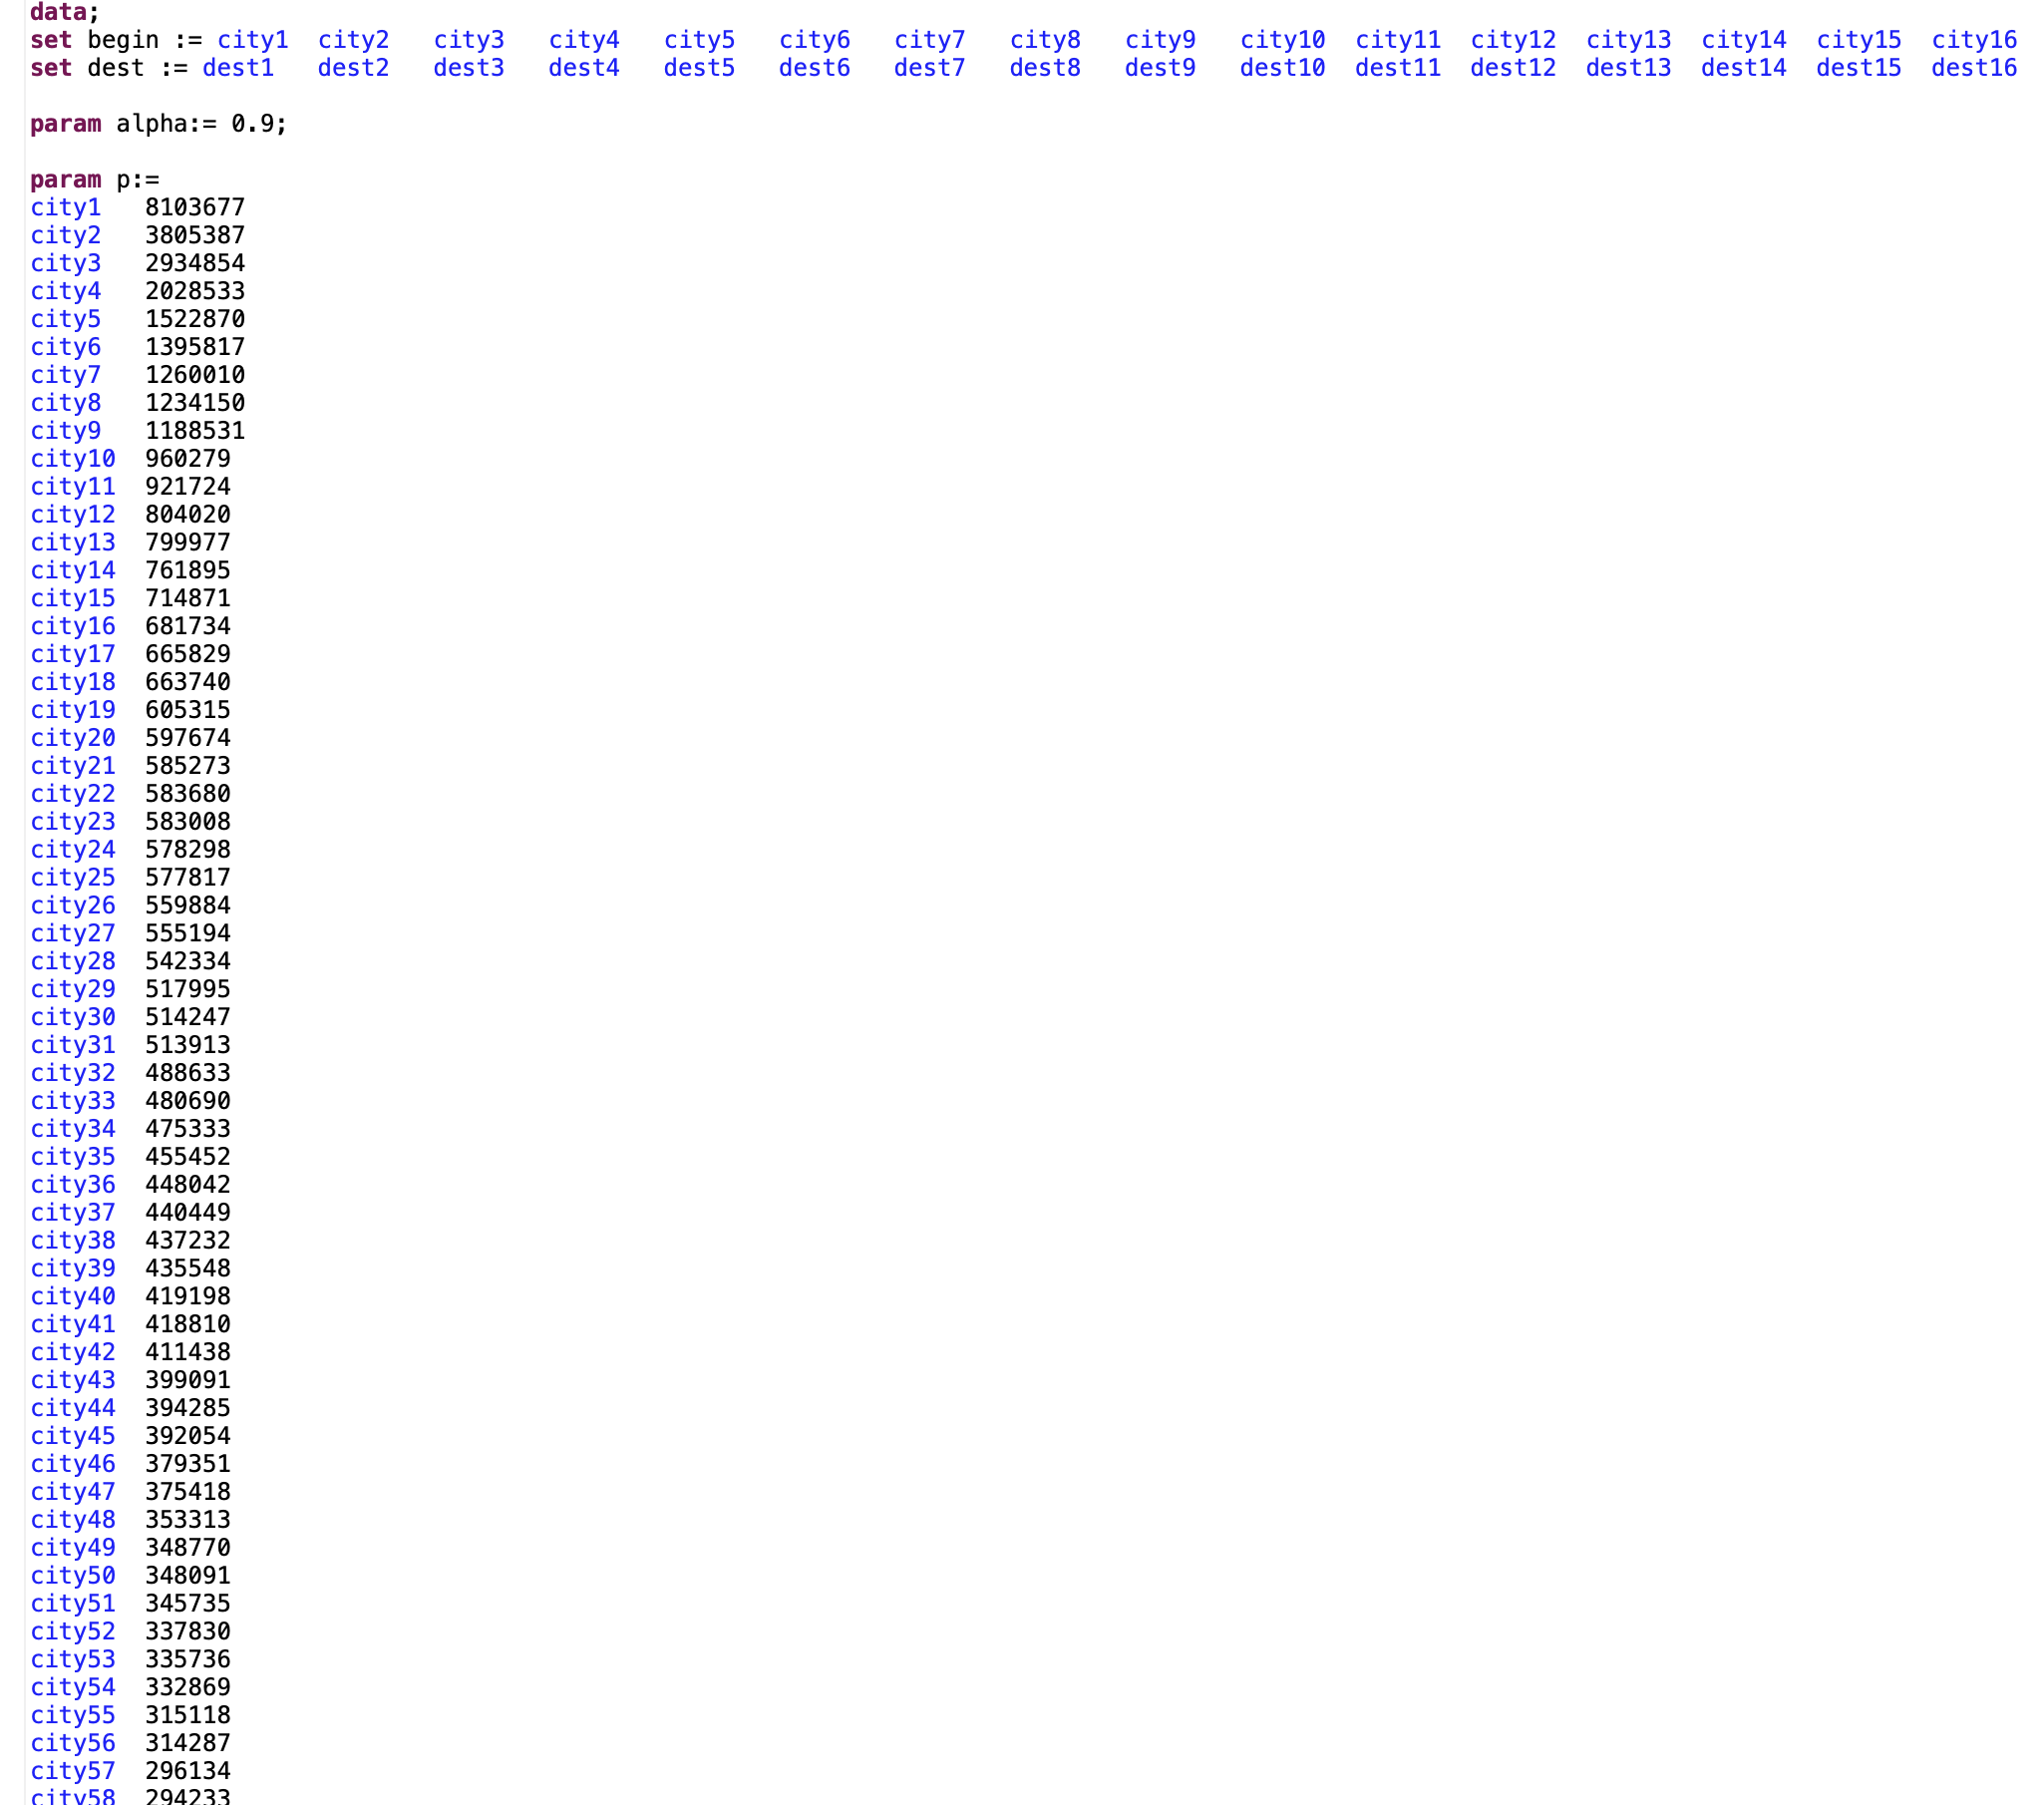
\includegraphics[width=0.55\linewidth]{fig2.png}
		\caption{.dat}
		\label{fig.prob1}
	\end{figure}
	\begin{figure}[H]
		\centering
		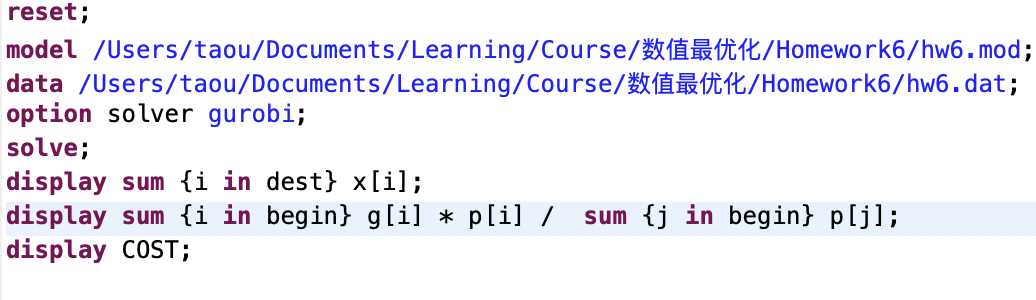
\includegraphics[width=0.55\linewidth]{fig3.png}
		\caption{.run}
		\label{fig.prob1}
	\end{figure}
	\begin{figure}[H]
		\centering
		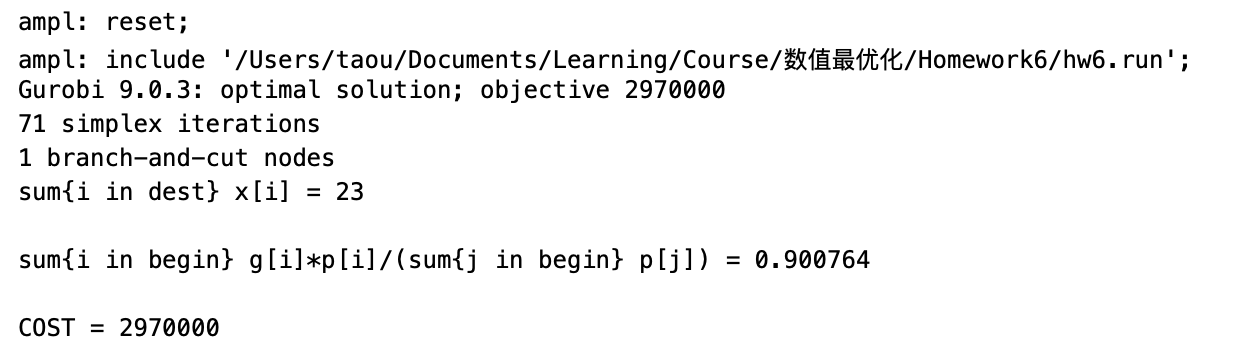
\includegraphics[width=0.55\linewidth]{fig4.png}
		\caption{result}
		\label{fig.prob1}
	\end{figure}
	\item 不接近。这个现象是非常正常的,因为在实际的建模过程中,我们的的目标函数与约束都会更加复杂,例如目标函数中我们还需要考虑运输成本,在约束中会加入DC容量的限制,等等。因此DC的数量和最低成本在直观上都会增加。
\end{enumerate}
\newpage
\section{\textbf{Solving the MX Problem}}
在上述问题$\bm{1}$中, 您制定了一个IP模型来解决MX的DC定点问题, 以确保给定的人口分数($\alpha$)在距离其最近的DC的$1$天邮寄范围内. 在此问题中, 您将开发一种基于Lagrangian松弛来求解此IP的方法.

作为出发点, 您要根据您的IP模型松弛某个约束, 并定义一个相应的乘子.
\begin{itemize}
	\item[$a)$] 写出这个松弛产生的Lagrangian子问题.~\textcolor{red}{[20pts]}
	
	\item[$b)$] 子问题应分解为两个分离的问题, 一个仅包含$\bm{x}$变量, 另一个仅包含$\bm{y}$变量. 写出这两个不同的问题.~\textcolor{red}{[20pts]}
	
	\item[$c)$] 请解释如何求解两个子问题, 即$\bm{x}$-子问题和$\bm{y}$-子问题. 您的求解方法可能不依赖于使用单纯型法或任何其他一般的LP或IP算法.~\textcolor{red}{[10pts]}
\end{itemize}
\begin{enumerate}
	\item 引入拉格朗日乘子$\lambda_i,\mu_i\ge 0$.
	\begin{equation}
		\begin{aligned}
			\min_{{\bf x},{\bf g}}\quad &\sum_{i=1}^n c_ix_i  + \sum_{i=1}^n\lambda_i(g_i-\sum_{j=1}^n x_j d_{ij}) + \sum_{i=1}^n\mu_i (\frac{\sum_{j=1}^n x_j d_{ij}}{1000}-g_i)\\
			s.t. \quad & \sum_{i=1}^n g_ip_i \ge \alpha \sum_{i=1}^n p_i \quad \text{(覆盖率达到$\alpha$)}\\
			\quad &x_{i}\in \{0,1\}, g_{i}\in \{0,1\} \quad \text{(整数约束)}\\
			\quad &\lambda,\mu \ge 0 
		\end{aligned}
	\end{equation}
	\item 将原问题分解为包含$x$和$g$的子问题:
	\begin{itemize}
		\item 	x-子问题\begin{equation}
		\begin{aligned}
			\min_{{\bf x}}\quad &\sum_{i=1}^n c_ix_i - \sum_{i=1}^n (\lambda_i-\frac{\mu_i}{1000})\sum_{j=1}^nx_jd_{ij} \\
			s.t. \quad &x_{i}\in \{0,1\},\lambda,\mu \ge 0
		\end{aligned}
	\end{equation}
	该形式可进一步化简为:
\begin{equation}
		\begin{aligned}
			\min_{{\bf x}}\quad &\sum_{i=1}^n \left(c_i-\sum_{j=1}^n(\lambda_j-\frac{\mu_j}{1000})d_{ji}\right) x_i  \\
			s.t. \quad &x_{i}\in \{0,1\},\lambda,\mu \ge 0
		\end{aligned}
	\end{equation}

	\item s-子问题
	\begin{equation}
		\begin{aligned}
			\min_{{\bf x}}\quad &\sum_{i=1}^n(\lambda_i-\frac{\mu_i}{1000})g_i \\
			s.t. \quad & \sum_{i=1}^n g_ip_i \ge \alpha \sum_{i=1}^n p_i \quad \text{(覆盖率达到$\alpha$)}\\ 
			\quad &g_{i}\in \{0,1\},\lambda,\mu \ge 0
		\end{aligned}
	\end{equation}
	\end{itemize}
	\item 
	\begin{itemize}
		\item 对于x-子问题:
			\begin{enumerate}
				\item 若$ c_i-\sum_{j=1}^n(\lambda_j-\frac{\mu_j}{1000})d_{ji}< 0$,则令$x_i=1$。
				\item 若$ c_i-\sum_{j=1}^n(\lambda_j-\frac{\mu_j}{1000})d_{ji}\ge 0$,则令$x_i=0$。
			\end{enumerate}
		\item 对于s-子问题:
			\begin{enumerate}
				\item 若$\lambda_i-\frac{\mu_i}{1000} < 0$,则令$g_i=1$,否则$g_i=0$。
				\item 如果得到的$x$满足约束,则该$x$即为最优解。
				\item 如果得到的$x$不满足约束,那么就依据$\lambda_i-\frac{\mu_i}{1000},\forall g_i = 0$的大小,从小到大依次将$g_i=0\rightarrow g_i=1$,直到约束满足为止。最终的$x'$即为最优解。
			\end{enumerate}
	\end{itemize}
\end{enumerate}
\end{document}